\subsection{Preventing traffic congestions for a one lane road}

A traffic congestions also known as traffic jams are when a long line of vehicles are moving slowly or have stopped moving completely. Traffic jams are annoying and distrupts nearby local environments with sound and gas emissions. There are many factors which can cause a traffic congestion such as:
poorly designed roads, not wide enough roads, traffic light patterns, and accidents. In conclusion, an event that distrupts the traffic flow can cause a traffic congestion.

With this in mind, we started by focusing on a simple scenario: when a car drasticly reduces their speed, or completely stops, in a single lane road. 

This scenario will lead to the vehicles behind needing to slow down as well, distrupting the traffic flow. To prevent this, the vehicles behind has to deacrease their velocity before they reach the destination of where the event happened. The reasoning for this is because then the vehicles does not need to decrease their velocity as drasticly. 

After a few dicussions in our group we came up with an idea of how the interactions between the server and the cars would be. First the car has to connect to the server and give information about its current speed, weight, width and lenght. The server would keep track on all the cars positions at the road. Since there is only a single road there was only one dimention to worry about. The cars would send information to the server if their velocity had changed. This would trigger an event on the server where it would tell all the cars behind the car that triggered the event to change their velocity to slow down accordingly. The velocity the cars would have to change to deppended on their distance to the car slowing down and their current velocity. Here is a flow chart of the demo for this solution:

\begin{figure}[h!]
	\centering
	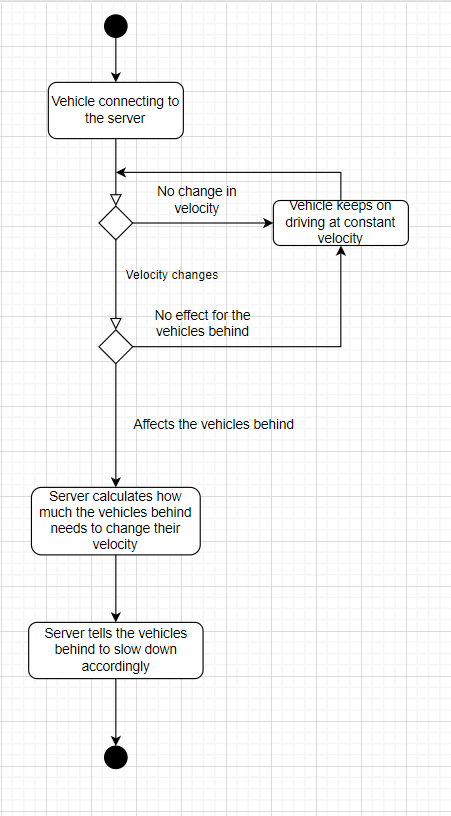
\includegraphics[width=1\linewidth]{figures/flow_diagram_first}
	\caption[Flow diagram server]{Flow diagram for the demo for the first solution.}
	\label{fig:diagramfirst}
\end{figure}